% ============================================================
%  Semana 10 · Clase 20: Regresión lineal con Python
%  Curso: Análisis y Visualización de Datos para la Toma de Decisiones
%
%  Formato de la sesión (3 h):
%    Hora 1. La idea de la regresión lineal: la recta, el ajuste por
%            mínimos cuadrados, leer los coeficientes y predecir
%    Hora 2. ¿Qué tan bien predice?: residuos, MAE, RMSE y R²; regresión
%            múltiple e interpretación de coeficientes
%    Hora 3. Límites del modelo y riesgos de extrapolación; presentación
%            de la práctica en dos rutas (Python y Orange)
%
%  Datos: datos/bicicletas_diarias.csv (Bike Sharing Dataset, UCI,
%  CC BY 4.0), generado con ../../../scripts/semana10-clase20_datos.py.
%  Figuras: figuras/*.pdf, con ../../../scripts/semana10-clase20_figuras.py.
%  Todas las cifras coinciden con el notebook y con la guía de Orange.
%
%  Compilar (dos veces) directamente desde esta carpeta:
%    xelatex semana10-clase20.tex
%    xelatex semana10-clase20.tex
% ============================================================
\documentclass[aspectratio=169,11pt]{beamer}

\usepackage{../../../plantilla/beamerthemeesumer}
\usetheme{esumer}

\usepackage[spanish,es-noshorthands]{babel}
\usepackage{booktabs}
\usepackage{graphicx}
\usepackage{array}
\newcolumntype{L}[1]{>{\raggedright\arraybackslash}p{#1}}
\newcolumntype{R}[1]{>{\raggedleft\arraybackslash}p{#1}}
\newcolumntype{C}[1]{>{\centering\arraybackslash}p{#1}}
\usetikzlibrary{arrows.meta,positioning,calc,decorations.pathreplacing}

% ---------------- DATOS DE LA CLASE ----------------
\title{Regresión lineal con Python}
\subtitle{Predecir un número y saber cuánto confiar en él}
\author{Docente: Cristian A. Jimenez C., MSc}
\date{Nov 10 al 15}

\setmodulo{Módulo 4: Innovar (Analítica Predictiva y Storytelling)}
\setsemana{10}
\setclase{20}
\setfechaclase{Nov 10 al 15}
\setmodalidad{Virtual}
% -----------------------------------------------------

\graphicspath{{figuras/}}

% Código en un recuadro sin título
\newcommand{\codigo}[1]{\par\smallskip\noindent\colorbox{esumerGray!70}{\parbox{\dimexpr\linewidth-2\fboxsep\relax}{\scriptsize\ttfamily #1}}\par\smallskip}

% Fuente de los datos, al pie
\newcommand{\fuentedatos}{\par\vspace{1pt}{\fontsize{5.5}{6.5}\selectfont\color{black!55}%
  Datos: Bike Sharing Dataset (Capital Bikeshare, Washington D.\,C.), UCI Machine Learning
  Repository, CC BY 4.0. Fanaee-T y Gama (2013).\par}}

\newcommand{\urluci}{https://archive.ics.uci.edu/dataset/275/bike+sharing+dataset}
\newcommand{\urlarticulo}{https://doi.org/10.1007/s13748-013-0040-3}
\newcommand{\urldatos}{https://github.com/craljimenez/An-lisis_y_Visualizacion_de_Datos_para_la_Toma_de_Decisiones/raw/main/clases/semana10-clase20-regresion-lineal-python/datos/bicicletas_diarias.csv}
\newcommand{\urlcolab}{https://colab.research.google.com/github/craljimenez/An-lisis_y_Visualizacion_de_Datos_para_la_Toma_de_Decisiones/blob/main/clases/semana10-clase20-regresion-lineal-python/notebooks/lab-regresion-lineal.ipynb}
\newcommand{\urlorange}{https://orangedatamining.com/download/}
\newcommand{\urlsklr}{https://scikit-learn.org/stable/modules/generated/sklearn.linear_model.LinearRegression.html}
\newcommand{\urlskmetricas}{https://scikit-learn.org/stable/modules/model_evaluation.html}
\newcommand{\urlolr}{https://orangedatamining.com/widget-catalog/model/linearregression/}
\newcommand{\urlislr}{https://www.statlearning.com/}

\begin{document}

{
\setbeamertemplate{footline}{}
\begin{frame}[plain,noframenumbering]
  \titlepage
\end{frame}
}

\begin{frame}[t]{Agenda de hoy (3 horas)}
  \begin{columns}[T,onlytextwidth]
    \column{0.32\textwidth}
    \begin{block}{Hora 1}
      \small La idea: una recta que sigue a los datos, cómo se ajusta, cómo
      se leen sus coeficientes y cómo predice.
    \end{block}
    \column{0.32\textwidth}
    \begin{block}{Hora 2}
      \small ¿Qué tan bien predice?: residuos, MAE, RMSE y $R^2$. Regresión
      múltiple y ``con lo demás igual''.
    \end{block}
    \column{0.32\textwidth}
    \begin{block}{Hora 3}
      \small Los límites del modelo y los riesgos de extrapolar. La
      práctica, en Python o en Orange.
    \end{block}
  \end{columns}
  \vspace{0.3cm}
  \small En la Clase 19 viste el mapa: si el objetivo es un número, la
  tarea es \textbf{regresión}; se entrena con unos datos, se prueba con
  otros y se compara con la \textbf{línea base}. Hoy construyes el modelo
  de regresión más sencillo y más usado, y aprendes a explicarlo en
  lenguaje de negocio.
\end{frame}

\begin{frame}[t]{Palabras nuevas de hoy}
  \footnotesize
  \renewcommand{\arraystretch}{1.18}
  \begin{tabular}{@{}L{3.4cm}L{10.1cm}@{}}
    \toprule
    \textbf{Regresión lineal} & Modelo que predice un número con una recta (o, con varias variables, un plano). \\
    \textbf{Intercepto y pendiente} & Los dos números que definen la recta: dónde corta el eje y cuánto sube por cada unidad de la variable. \\
    \textbf{Coeficiente} & El número que multiplica a cada variable explicativa. La pendiente es un coeficiente. \\
    \textbf{Residuo} & Lo real menos lo predicho, en cada caso. Es el error del modelo en ese caso. \\
    \textbf{Mínimos cuadrados} & La regla para elegir la recta: la que hace más pequeña la suma de los residuos al cuadrado. \\
    \textbf{MAE, RMSE, $R^2$} & Tres formas de medir qué tan bien predice el modelo. \\
    \textbf{Extrapolar} & Predecir fuera del rango de los datos con que aprendió el modelo. \\
    \bottomrule
  \end{tabular}
\end{frame}

% ============================================================
\section{Hora 1: La idea de la regresión lineal}
% ============================================================
\begin{frame}[t]{El caso de hoy: ¿cuántas bicicletas preparar?}
  \begin{columns}[T,onlytextwidth]
    \column{0.52\textwidth}
    \small
    \textbf{Capital Bikeshare} alquila bicicletas en Washington D.\,C. Cada
    noche decide cuántas bicicletas y cuánto personal tener listos para el
    día siguiente.
    \vspace{0.15cm}

    Tenemos \textbf{731 días reales} (2011 y 2012): cuántas bicicletas se
    alquilaron y el clima de cada día.
    \vspace{0.15cm}
    \begin{exampleblock}{La pregunta predictiva (Clase 19)}
      \footnotesize \textbf{Para decidir} cuántas bicicletas y personas
      preparar, \textbf{quiero predecir} los alquileres \textbf{de cada}
      día, \textbf{usando} el pronóstico del clima y el calendario,
      \textbf{con anticipación} de un día.
    \end{exampleblock}
    \column{0.44\textwidth}
    \footnotesize
    \renewcommand{\arraystretch}{1.15}
    \begin{tabular}{@{}L{2.5cm}L{3.2cm}@{}}
      \toprule
      \textbf{Columna} & \textbf{Rol} \\
      \midrule
      \texttt{alquileres} & Objetivo $y$ (un número) \\
      \texttt{temperatura\_c} & Explicativa \\
      \texttt{humedad}, \texttt{viento} & Explicativas \\
      \texttt{lluvia} (0 o 1) & Explicativa \\
      \texttt{es\_2012} (0 o 1) & Explicativa \\
      \texttt{dia\_laboral} (0 o 1) & Explicativa \\
      \textit{Reparto} & 80\% entrenamiento (584 días) y 20\% prueba (147) \\
      \bottomrule
    \end{tabular}
  \end{columns}
  \fuentedatos
\end{frame}

\begin{frame}[t]{Antes de modelar, mirar}
  \begin{columns}[T,onlytextwidth]
    \column{0.6\textwidth}
    \centering
    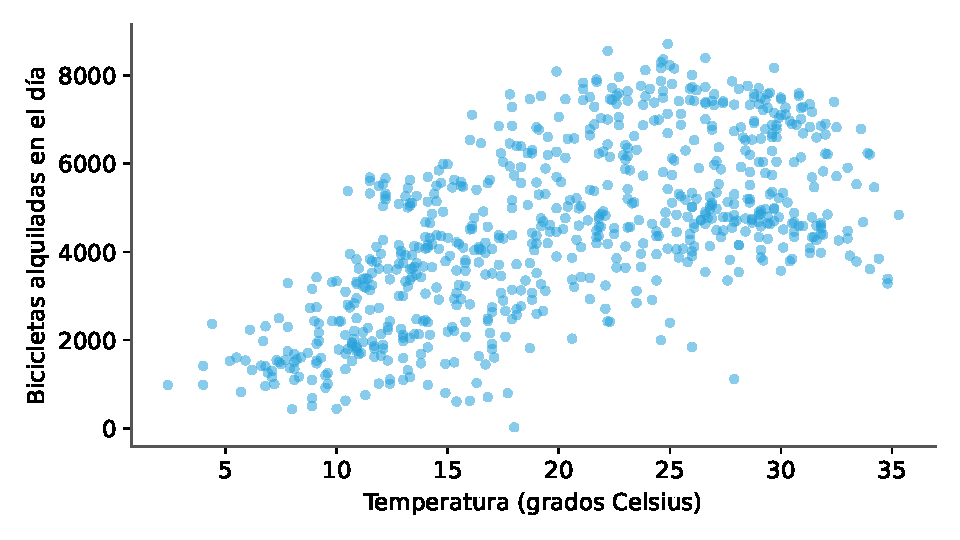
\includegraphics[width=\linewidth,height=5.1cm,keepaspectratio]{fig_dispersion.pdf}
    \column{0.37\textwidth}
    \small
    Cada punto es un día. Con más temperatura hay más alquileres: la
    correlación es \textbf{0,627}, positiva y moderada (Clase 11).
    \vspace{0.15cm}

    La regresión lineal supone que la relación es, más o menos, una
    \textbf{recta}. Mira con cuidado la derecha: en los días más calurosos
    la nube deja de subir. Volveremos a eso.
    \vspace{0.15cm}
    \begin{block}{Regla}
      \footnotesize Nunca ajustes un modelo sin haber mirado antes el
      gráfico de dispersión.
    \end{block}
  \end{columns}
  \fuentedatos
\end{frame}

\begin{frame}[t]{La idea: una recta}
  \begin{columns}[T,onlytextwidth]
    \column{0.5\textwidth}
    \centering
    \begin{tikzpicture}[x=0.9cm, y=0.9cm]
      \draw[-{Stealth[length=2mm]}, esumerNavy] (0,0) -- (6,0) node[below left, font=\scriptsize, text=black] {$x$: temperatura};
      \draw[-{Stealth[length=2mm]}, esumerNavy] (0,0) -- (0,4.4) node[above right, font=\scriptsize, text=black] {$y$: alquileres};
      \draw[esumerOrange, line width=1.6pt] (0,0.9) -- (5.6,3.9);
      \fill[esumerNavy] (0,0.9) circle (2.2pt);
      \node[font=\scriptsize, text=esumerNavy, anchor=east] at (-0.1,0.9) {$b_0$};
      \draw[esumerTeal, line width=1pt] (2.5,2.24) -- (3.5,2.24) -- (3.5,2.78);
      \node[font=\scriptsize, text=esumerTeal, below] at (3.0,2.24) {+1 grado};
      \node[font=\scriptsize, text=esumerTeal, right] at (3.5,2.51) {+$b_1$ bicicletas};
    \end{tikzpicture}
    \column{0.47\textwidth}
    \small
    \[ \hat{y} = b_0 + b_1 \cdot x \]
    \begin{itemize}
      \small
      \item $\hat{y}$ (``y gorro''): la \textbf{predicción}.
      \item $b_0$, el \textbf{intercepto}: el valor de la recta cuando
        $x$ es 0.
      \item $b_1$, la \textbf{pendiente}: cuánto cambia $\hat{y}$ cuando
        $x$ sube en 1.
    \end{itemize}
    \vspace{0.1cm}
    \footnotesize Ajustar el modelo es \textbf{encontrar $b_0$ y $b_1$} a
    partir de los datos de entrenamiento. Todo lo demás (predecir, medir,
    explicar) sale de esos dos números.
  \end{columns}
\end{frame}

\begin{frame}[t]{¿Cuál recta? Mínimos cuadrados}
  \begin{columns}[T,onlytextwidth]
    \column{0.47\textwidth}
    \centering
    \begin{tikzpicture}[x=0.85cm, y=0.85cm]
      \draw[-{Stealth[length=2mm]}, esumerNavy] (0,0) -- (6,0);
      \draw[-{Stealth[length=2mm]}, esumerNavy] (0,0) -- (0,4.2);
      \draw[esumerOrange, line width=1.4pt] (0.2,0.8) -- (5.8,3.6);
      \foreach \x/\y in {0.7/1.6, 1.4/0.7, 2.1/2.0, 2.8/1.6, 3.5/2.9, 4.2/2.2, 4.9/3.7, 5.5/3.0}
        {\draw[esumerTeal, line width=1pt] (\x,\y) -- (\x,{0.8+(\x-0.2)*0.5});
         \fill[esumerSky] (\x,\y) circle (2.6pt);}
      \node[font=\scriptsize, text=esumerTeal, align=left, anchor=west] at (1.5,3.9) {residuos:\\real menos predicho};
    \end{tikzpicture}

    {\scriptsize\color{black!60}Esquema; los puntos no son datos reales.}
    \column{0.5\textwidth}
    \small
    Hay infinitas rectas posibles. Cada una deja una distancia vertical
    entre cada punto y la recta: el \textbf{residuo}.
    \vspace{0.1cm}

    La regresión lineal elige la recta que hace más pequeña la
    \textbf{suma de los residuos al cuadrado}. Por eso se llama de
    \textbf{mínimos cuadrados}.
    \vspace{0.1cm}
    \begin{block}{¿Por qué al cuadrado?}
      \footnotesize Para que los residuos positivos y negativos no se
      cancelen, y para castigar más los errores grandes. No lo calculas tú:
      lo hace \texttt{LinearRegression()} en Python o el widget
      \textbf{Linear Regression} en Orange.
    \end{block}
  \end{columns}
\end{frame}

\begin{frame}[t]{La recta de nuestros datos}
  \begin{columns}[T,onlytextwidth]
    \column{0.58\textwidth}
    \centering
    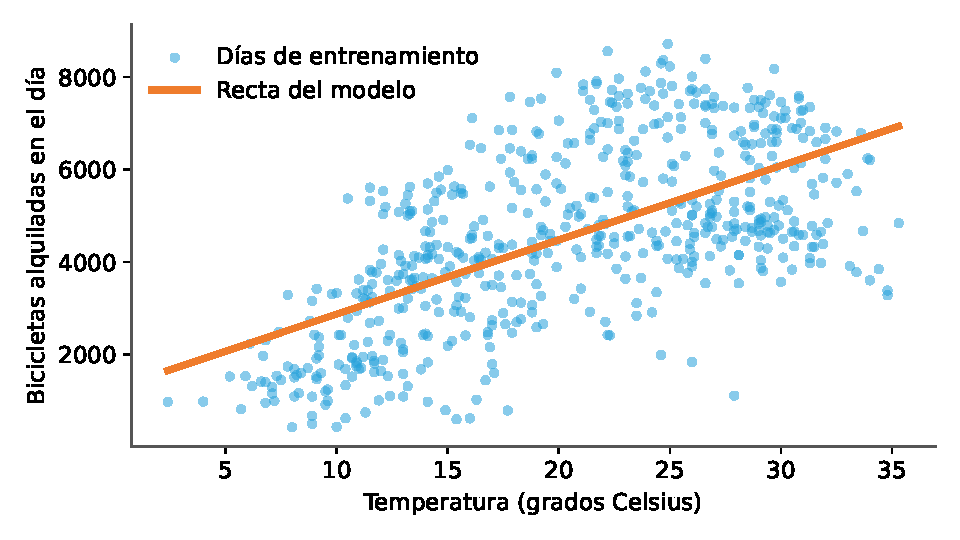
\includegraphics[width=\linewidth,height=5.0cm,keepaspectratio]{fig_recta.pdf}
    \column{0.39\textwidth}
    \small Con los 584 días de entrenamiento:
    \[ \hat{y} = 1272{,}76 + 160{,}35 \cdot \text{temperatura} \]
    \footnotesize En Python:
    \codigo{modelo = LinearRegression()\\
      modelo.fit(X\_train, y\_train)\\[2pt]
      modelo.intercept\_\ \ \ \# 1272.76\\
      modelo.coef\_\ \ \ \ \ \ \ \# [160.35]}
    \footnotesize En Orange: widget \textbf{Linear Regression}, salida
    \textbf{Coefficients}.
  \end{columns}
  \fuentedatos
\end{frame}

\begin{frame}[t]{Leer los coeficientes en lenguaje de negocio}
  \small
  Un coeficiente no se entrega como un número suelto: se traduce a la
  decisión.
  \vspace{0.1cm}
  \footnotesize
  \renewcommand{\arraystretch}{1.3}
  \begin{tabular}{@{}L{2.5cm}L{4.5cm}L{6.1cm}@{}}
    \toprule
    & \textbf{Así no} & \textbf{Así sí} \\
    \midrule
    \textbf{Pendiente} 160,35 & ``El coeficiente de temperatura es 160,35.'' & ``Por cada grado más de temperatura, se alquilan en promedio unas \textbf{160 bicicletas más} al día.'' \\
    \textbf{Intercepto} 1272,76 & ``A 0 grados se alquilan 1273 bicicletas.'' & No se lee como predicción: ningún día de los datos llegó a 0 grados (el más frío tuvo 2,4). Solo fija la altura de la recta. \\
    \bottomrule
  \end{tabular}
  \vspace{0.2cm}
  \begin{columns}[T,onlytextwidth]
    \column{0.48\textwidth}
    \begin{block}{Las unidades importan}
      \footnotesize La pendiente está en \textbf{bicicletas por grado}. Si
      la temperatura estuviera en grados Fahrenheit, el número cambiaría,
      aunque la relación sea la misma.
    \end{block}
    \column{0.48\textwidth}
    \begin{alertblock}{Promedio, no certeza}
      \footnotesize ``En promedio'' es parte de la frase: un día concreto
      puede quedar muy lejos de la recta.
    \end{alertblock}
  \end{columns}
\end{frame}

\begin{frame}[t]{Predecir con la recta}
  \small
  Para un día de 25 grados, se reemplaza en la ecuación:
  \[ \hat{y} = 1272{,}76 + 160{,}35 \times 25 = 5281 \text{ bicicletas} \]
  \begin{columns}[T,onlytextwidth]
    \column{0.48\textwidth}
    \footnotesize\textbf{En Python}
    \codigo{dia = pd.DataFrame(\{"temperatura\_c": [25]\})\\
      modelo.predict(dia)\ \ \ \# array([5281.4])}
    \column{0.48\textwidth}
    \footnotesize\textbf{En Orange}
    \par\smallskip
    \footnotesize Widget \textbf{Create Instance} con
    \texttt{temperatura\_c} = 25, conectado con \textbf{Predictions} junto
    al modelo.
  \end{columns}
  \vspace{0.15cm}
  \begin{alertblock}{¿5281 es lo que va a pasar?}
    \footnotesize Es lo que la recta dice para un día \emph{típico} de 25
    grados. Para saber cuánto confiar en esa cifra hay que medir cuánto se
    equivoca el modelo: es la Hora 2.
  \end{alertblock}
\end{frame}

% ============================================================
\section{Hora 2: ¿Qué tan bien predice?}
% ============================================================
\begin{frame}[t]{Los residuos, día por día}
  \small
  Tres días reales de entrenamiento, con el modelo de la temperatura:
  \vspace{0.1cm}
  \footnotesize
  \renewcommand{\arraystretch}{1.2}
  \begin{tabular}{@{}L{3.6cm}R{1.8cm}R{1.7cm}R{1.9cm}R{1.7cm}@{}}
    \toprule
    \textbf{Día} & \textbf{Temperatura} & \textbf{Real} & \textbf{Predicho} & \textbf{Residuo} \\
    \midrule
    miércoles 5 ene.\ 2011 & 9,3 & 1600 & 2764 & $-1164$ \\
    lunes 25 jul.\ 2011 & 30,5 & 3840 & 6163 & $-2323$ \\
    sábado 22 sep.\ 2012 & 26,6 & 8395 & 5538 & $+2857$ \\
    \bottomrule
  \end{tabular}
  \vspace{0.15cm}
  \begin{columns}[T,onlytextwidth]
    \column{0.48\textwidth}
    \begin{block}{Cómo se leen}
      \footnotesize Residuo negativo: el modelo predijo \textbf{de más}.
      Positivo: \textbf{de menos}. El 22 de septiembre de 2012 se alquilaron
      casi 2900 bicicletas más de lo previsto.
    \end{block}
    \column{0.48\textwidth}
    \begin{block}{Para qué sirven}
      \footnotesize Los residuos son la parte que el modelo
      \textbf{no explica}. De ellos salen las medidas de error y, mirados
      en un gráfico, sus límites.
    \end{block}
  \end{columns}
\end{frame}

\begin{frame}[t]{Tres medidas del error}
  \footnotesize
  \renewcommand{\arraystretch}{1.25}
  \begin{tabular}{@{}L{1.3cm}L{5.3cm}L{6.5cm}@{}}
    \toprule
    & \textbf{Qué es} & \textbf{Cómo se lee} \\
    \midrule
    \textbf{MAE} & Promedio de los residuos en valor absoluto. & ``En promedio, el modelo se equivoca en tantas bicicletas.'' La más fácil de explicar. \\
    \textbf{RMSE} & Raíz del promedio de los residuos al cuadrado. & También en bicicletas, pero castiga más los errores grandes. Siempre es mayor o igual que el MAE. \\
    \textbf{$R^2$} & $1 - \dfrac{\text{suma de residuos}^2}{\text{suma de distancias al promedio}^2}$ & Qué parte de la variación explica el modelo. 1 es perfecto; 0 es lo mismo que predecir el promedio. \\
    \bottomrule
  \end{tabular}
  \vspace{0.15cm}

  \small\textbf{Con los 147 días de prueba}, que el modelo no vio:
  \vspace{0.05cm}

  \footnotesize
  \begin{tabular}{@{}L{5.0cm}R{1.8cm}R{1.8cm}R{1.6cm}@{}}
    \toprule
    \textbf{Modelo} & \textbf{MAE} & \textbf{RMSE} & \textbf{$R^2$} \\
    \midrule
    Línea base (siempre el promedio) & 1712,0 & 2022,2 & $-0{,}020$ \\
    Simple (temperatura) & 1291,7 & 1545,9 & 0,404 \\
    \bottomrule
  \end{tabular}
\end{frame}

\begin{frame}[t]{El $R^2$ es orientativo}
  \begin{columns}[T,onlytextwidth]
    \column{0.5\textwidth}
    \small
    Nuestro modelo simple tiene $R^2$ de \textbf{0,388} con los días de
    entrenamiento y de \textbf{0,404} con los de prueba.
    \vspace{0.1cm}

    \footnotesize Son parecidos: buena señal de que el modelo no memorizó
    (Clase 19). Si el de prueba fuera mucho más bajo, habría sobreajuste. El
    que se reporta es el de \textbf{prueba}.
    \vspace{0.15cm}
    \begin{block}{¿Es bueno un $R^2$ de 0,40?}
      \footnotesize Depende de la decisión. Para planear bicicletas, mejora
      a la línea base en unas 420 bicicletas diarias de error, pero deja
      cerca del 60\% de la variación sin explicar.
    \end{block}
    \column{0.46\textwidth}
    \begin{alertblock}{Tres errores comunes}
      \footnotesize
      \begin{itemize}
        \footnotesize
        \item Creer que hay un $R^2$ ``mínimo aceptable'' para todo.
        \item Creer que un $R^2$ alto prueba una causa (Clase 19).
        \item Mirar solo el $R^2$: un modelo puede tener $R^2$ aceptable y
          fallar siempre en el mismo tipo de días. Para eso están los
          residuos.
      \end{itemize}
    \end{alertblock}
    \footnotesize Por eso se reporta siempre junto al \textbf{MAE}, que dice
    el error en las unidades del negocio.
  \end{columns}
\end{frame}

\begin{frame}[t]{Los residuos tienen forma: la relación no es recta}
  \begin{columns}[T,onlytextwidth]
    \column{0.58\textwidth}
    \centering
    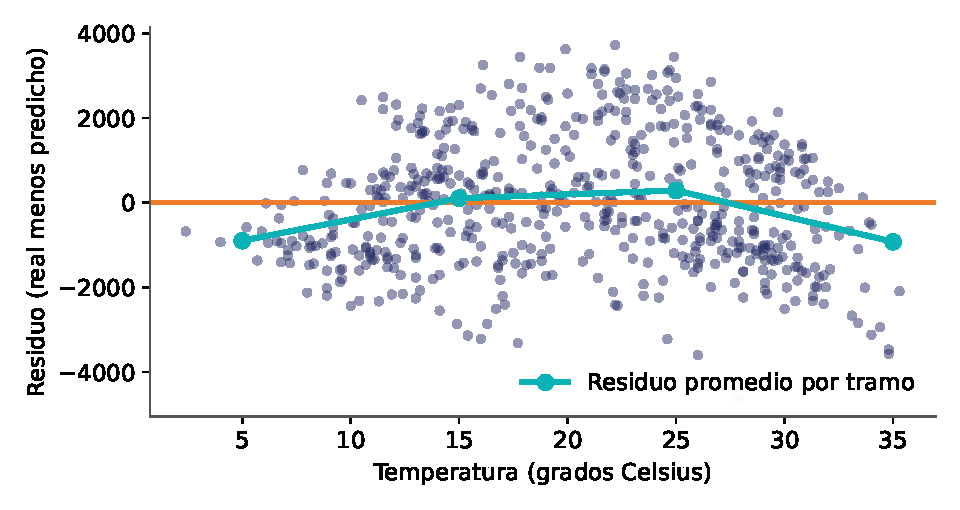
\includegraphics[width=\linewidth,height=4.9cm,keepaspectratio]{fig_residuos.pdf}
    \column{0.39\textwidth}
    \small
    Si el modelo fuera adecuado, los residuos quedarían al azar alrededor
    de cero. Aquí forman un \textbf{arco}:
    \vspace{0.05cm}

    \footnotesize
    \renewcommand{\arraystretch}{1.1}
    \begin{tabular}{@{}L{2.4cm}R{1.8cm}@{}}
      \toprule
      \textbf{Temperatura} & \textbf{Residuo prom.} \\
      \midrule
      0 a 10 & $-897$ \\
      10 a 20 & $107$ \\
      20 a 30 & $290$ \\
      30 a 40 & $-923$ \\
      \bottomrule
    \end{tabular}
    \vspace{0.1cm}

    \footnotesize Con frío y con calor fuerte, predice de más. Una recta no
    puede doblarse: es un \textbf{límite del modelo}, no un error tuyo.
  \end{columns}
  \fuentedatos
\end{frame}

\begin{frame}[t]{Regresión lineal múltiple}
  \small
  Con varias variables explicativas, la idea es la misma: un coeficiente
  por variable.
  \[ \hat{y} = b_0 + b_1 \cdot \text{temperatura} + b_2 \cdot \text{humedad} + \cdots + b_6 \cdot \text{lluvia} \]
  \begin{columns}[T,onlytextwidth]
    \column{0.5\textwidth}
    \begin{block}{``Con lo demás igual''}
      \footnotesize Cada coeficiente es el cambio en la predicción cuando
      esa variable sube en 1 y \textbf{las demás se mantienen fijas}. Es lo
      que hace útil a la regresión múltiple: separa el efecto de cada
      variable.
    \end{block}
    \column{0.46\textwidth}
    \begin{block}{Variables de 0 y 1}
      \footnotesize En \texttt{lluvia}, pasar de 0 a 1 es pasar de un día
      seco a uno con lluvia: su coeficiente es la diferencia entre los dos
      tipos de día.
    \end{block}
  \end{columns}
  \vspace{0.1cm}
  \footnotesize Las variables se eligen con las preguntas de la Clase 19:
  ¿las tendré al momento de predecir?, ¿aportan?, ¿repiten lo que dice
  otra? Por eso no usamos la sensación térmica: su correlación con la
  temperatura es de 0,99.
\end{frame}

\begin{frame}[t]{El modelo múltiple, en lenguaje de negocio}
  \footnotesize
  \renewcommand{\arraystretch}{1.12}
  \begin{tabular}{@{}L{2.6cm}R{1.6cm}L{8.9cm}@{}}
    \toprule
    \textbf{Variable} & \textbf{Coeficiente} & \textbf{Con lo demás igual\ldots} \\
    \midrule
    intercepto & 2070,77 & \\
    \texttt{temperatura\_c} & 152,56 & cada grado más, unas 153 bicicletas más al día. \\
    \texttt{humedad} & $-16{,}75$ & cada punto más de humedad, unas 17 menos. \\
    \texttt{viento} & $-51{,}17$ & cada punto más de viento, unas 51 menos. \\
    \texttt{es\_2012} & 1959,94 & un día de 2012 tiene unas 1960 más que uno parecido de 2011. \\
    \texttt{dia\_laboral} & 145,40 & un día laboral tiene unas 145 más: poca diferencia. \\
    \texttt{lluvia} & $-1239{,}71$ & un día con lluvia o nieve, unas 1240 menos. \\
    \bottomrule
  \end{tabular}
  \vspace{0.12cm}
  \begin{columns}[T,onlytextwidth]
    \column{0.48\textwidth}
    \begin{block}{La temperatura bajó de 160 a 153}
      \footnotesize Parte de lo que el modelo simple le atribuía era, en
      realidad, del año o de la lluvia.
    \end{block}
    \column{0.48\textwidth}
    \begin{alertblock}{Grande no es importante}
      \footnotesize Los coeficientes dependen de las unidades: un punto de
      humedad no se compara con pasar de 2011 a 2012.
    \end{alertblock}
  \end{columns}
\end{frame}

\begin{frame}[t]{¿Valió la pena agregar variables?}
  \small
  Los tres modelos, con los mismos 147 días de prueba:
  \vspace{0.1cm}

  \footnotesize
  \renewcommand{\arraystretch}{1.2}
  \begin{tabular}{@{}L{5.2cm}R{1.8cm}R{1.8cm}R{1.6cm}@{}}
    \toprule
    \textbf{Modelo} & \textbf{MAE} & \textbf{RMSE} & \textbf{$R^2$} \\
    \midrule
    Línea base (siempre el promedio) & 1712,0 & 2022,2 & $-0{,}020$ \\
    Simple (temperatura) & 1291,7 & 1545,9 & 0,404 \\
    Múltiple (6 variables) & \textbf{733,4} & \textbf{919,1} & \textbf{0,789} \\
    \bottomrule
  \end{tabular}
  \vspace{0.2cm}

  \begin{columns}[T,onlytextwidth]
    \column{0.48\textwidth}
    \begin{exampleblock}{El mensaje para la gerencia}
      \footnotesize ``Con el pronóstico del clima y el calendario, el error
      diario baja de unas 1700 bicicletas a unas 730: \textbf{menos de la mitad}.''
    \end{exampleblock}
    \column{0.48\textwidth}
    \begin{block}{Y una predicción concreta}
      \footnotesize Un día laboral de 2012, a 25 grados, humedad 60, viento
      12: unas \textbf{6371} bicicletas sin lluvia y \textbf{5131} con
      lluvia, con un error típico de unas 730.
    \end{block}
  \end{columns}
\end{frame}

% ============================================================
\section{Hora 3: Los límites del modelo}
% ============================================================
\begin{frame}[t]{Extrapolar: predecir fuera de los datos}
  \begin{columns}[T,onlytextwidth]
    \column{0.58\textwidth}
    \centering
    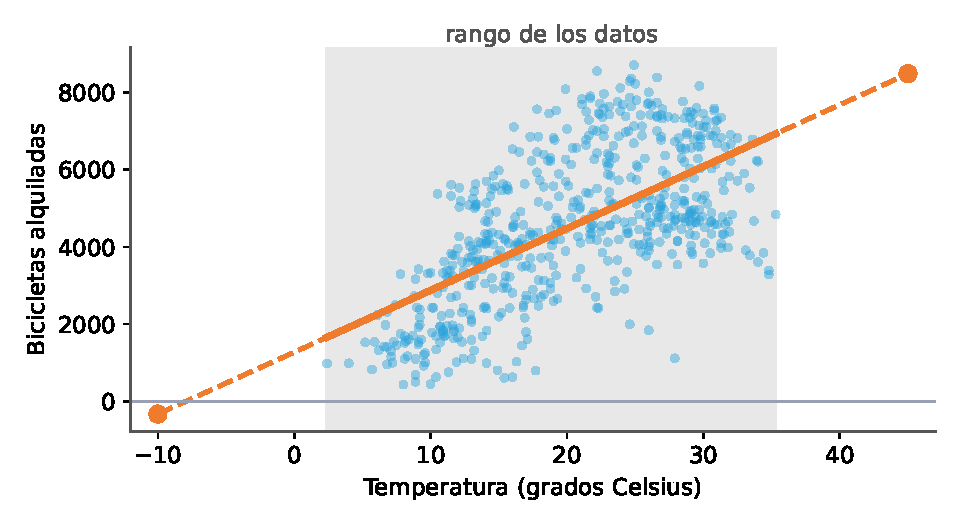
\includegraphics[width=\linewidth,height=5.0cm,keepaspectratio]{fig_extrapolacion.pdf}
    \column{0.39\textwidth}
    \small
    El modelo aprendió con días entre \textbf{2,4 y 35,3 grados} (zona
    gris). Fuera de ella, la recta sigue sin freno:
    \begin{itemize}
      \footnotesize
      \item A $-10$ grados predice \textbf{$-331$} bicicletas: un número
        imposible.
      \item A 45 grados predice \textbf{8488}, aunque los datos muestran
        que con calor fuerte los alquileres bajan.
    \end{itemize}
    \begin{alertblock}{Regla}
      \footnotesize Usa el modelo solo dentro del rango de los datos con que
      aprendió, y para situaciones parecidas a las que vio.
    \end{alertblock}
  \end{columns}
  \fuentedatos
\end{frame}

\begin{frame}[t]{Lo que el modelo no ve}
  \small
  Los días de prueba en que más se equivocó el modelo múltiple:
  \vspace{0.1cm}

  \footnotesize
  \renewcommand{\arraystretch}{1.2}
  \begin{tabular}{@{}L{2.2cm}L{2.8cm}R{1.2cm}R{1.5cm}L{4.6cm}@{}}
    \toprule
    \textbf{Fecha} & \textbf{Clima} & \textbf{Real} & \textbf{Predicho} & \textbf{Qué pasó} \\
    \midrule
    29 oct.\ 2012 & Lluvia, 18 grados & 22 & 2980 & Llegó el huracán Sandy a la costa este de EE.\,UU. \\
    29 jun.\ 2012 & Despejado, 34,2 grados & 5463 & 8006 & Calor fuerte, que la recta no captura. \\
    \bottomrule
  \end{tabular}
  \vspace{0.15cm}
  \begin{columns}[T,onlytextwidth]
    \column{0.48\textwidth}
    \begin{block}{Eventos que no están en las columnas}
      \footnotesize Ningún dato del clima diario anticipa una ciudad
      cerrada por un huracán. Un modelo solo sabe lo que hay en sus
      variables.
    \end{block}
    \column{0.48\textwidth}
    \begin{exampleblock}{No escondas estos casos}
      \footnotesize Explicarlos da confianza: muestra que sabes dónde
      funciona el modelo y dónde no. Van en tu presentación.
    \end{exampleblock}
  \end{columns}
\end{frame}

\begin{frame}[t]{Otros tres riesgos}
  \footnotesize
  \renewcommand{\arraystretch}{1.3}
  \begin{tabular}{@{}L{3.0cm}L{5.3cm}L{4.8cm}@{}}
    \toprule
    \textbf{Riesgo} & \textbf{En nuestros datos} & \textbf{Qué hacer} \\
    \midrule
    \textbf{Leer un coeficiente como causa} & \texttt{es\_2012} suma 1960 bicicletas. No es que el año cause alquileres: el uso del sistema creció de un año a otro. & Decir ``se asocia con'', no ``causa'', salvo que haya un experimento (Clase 19). \\
    \textbf{Variables que repiten lo mismo} & Si agregas la sensación térmica, el coeficiente de la temperatura cae de 153 a 63 y el MAE apenas cambia (de 733,4 a 729,6). & Quitar una de las dos. Los coeficientes de variables redundantes no se pueden leer. \\
    \textbf{El negocio cambia} & En 2012 el promedio diario fue de 5600 alquileres; en 2011, de 3406. & Volver a entrenar con datos recientes y vigilar el error mes a mes. \\
    \bottomrule
  \end{tabular}
\end{frame}

\begin{frame}[t]{Antes de presentar un modelo de regresión}
  \begin{columns}[T,onlytextwidth]
    \column{0.55\textwidth}
    \small
    \begin{enumerate}
      \small
      \item Miré el gráfico de dispersión antes de ajustar.
      \item Medí con datos de \textbf{prueba}, no de entrenamiento.
      \item Comparé con la \textbf{línea base}.
      \item Reporto el \textbf{MAE} en unidades del negocio, junto al $R^2$.
      \item Revisé los \textbf{residuos}: ¿tienen forma?
      \item Expliqué cada coeficiente con ``con lo demás igual''.
      \item Dije el \textbf{rango} en que vale el modelo.
      \item Expliqué los casos en que más se equivoca.
    \end{enumerate}
    \column{0.41\textwidth}
    \begin{exampleblock}{Una frase completa}
      \footnotesize ``Con el pronóstico del clima y el calendario, podemos
      anticipar los alquileres del día con un error típico de unas 730
      bicicletas. La lluvia los reduce en unas 1200. El modelo vale para
      días entre 2 y 35 grados y no anticipa eventos extraordinarios, como
      un huracán.''
    \end{exampleblock}
  \end{columns}
\end{frame}

% ============================================================
\section{Práctica}
% ============================================================
\begin{frame}[t]{La práctica: elige tu ruta}
  \begin{columns}[T,onlytextwidth]
    \column{0.48\textwidth}
    \begin{block}{Ruta Python}
      \footnotesize Notebook \texttt{lab-regresion-lineal.ipynb}, en Google
      Colab. Usa pandas y scikit-learn, como en los Módulos 1 y 2.\\[3pt]
      \href{\urlcolab}{\color{esumerOrange}Abrir en Colab}
    \end{block}
    \column{0.48\textwidth}
    \begin{block}{Ruta Orange}
      \footnotesize Guía \texttt{guia-orange-regresion-lineal.pdf}. Sin
      código: arrastras widgets y los conectas (Clase 19).\\[3pt]
      \href{\urlorange}{\color{esumerOrange}Descargar Orange}
    \end{block}
  \end{columns}
  \vspace{0.2cm}
  \small Las dos rutas tienen \textbf{los mismos nueve pasos}. Cada una
  reparte los días con su herramienta habitual, con la misma semilla:
  \texttt{train\_test\_split(test\_size=0.2, random\_state=42)} en Python y
  \textbf{Data Sampler} al 20\% con muestreo replicable en Orange. Eligen los
  mismos días, así que \textbf{las cifras salen idénticas}. Cada paso termina con una caja
  ``Debes ver'' para comprobar que vas bien.
  \vspace{0.1cm}

  \footnotesize
  \renewcommand{\arraystretch}{1.1}
  \begin{tabular}{@{}L{0.5cm}L{5.7cm}L{0.5cm}L{6.0cm}@{}}
    1 & Cargar y revisar los datos & 6 & Los residuos \\
    2 & Mirar la relación & 7 & Regresión múltiple \\
    3 & Separar entrenamiento y prueba & 8 & Predecir un día nuevo \\
    4 & La línea base & 9 & Los límites del modelo \\
    5 & Regresión simple & & \\
  \end{tabular}
\end{frame}

\begin{frame}[t]{Producto esperado}
  \small
  Al final de la práctica entregas la \textbf{ficha en lenguaje de negocio}
  (está al final del notebook y de la guía):
  \vspace{0.1cm}
  \begin{enumerate}
    \small
    \item ¿Qué decisión apoya el modelo?
    \item ¿Cuánto mejora a la línea base? (MAE de la base y del modelo)
    \item ¿Qué dos coeficientes le contarías a la gerencia, y cómo los
      dirías?
    \item ¿En qué días se equivoca más, y por qué?
    \item ¿Qué no debe hacerse con este modelo?
  \end{enumerate}
  \vspace{0.1cm}
  \begin{block}{Si trabajas en pareja}
    \footnotesize Uno en Python y otro en Orange: comparen las cifras de
    cada paso. Si no coinciden, el error está en uno de los dos, y
    encontrarlo es parte del aprendizaje.
  \end{block}
\end{frame}

% ============================================================
\section{Cierre}
% ============================================================
\begin{frame}[t]{Cierre y próxima sesión}
  \begin{itemize}
    \footnotesize
    \item La regresión lineal predice un número con una recta:
      $\hat{y} = b_0 + b_1 x$. Ajustarla es encontrar los coeficientes que
      hacen mínima la suma de los residuos al cuadrado.
    \item Cada coeficiente se dice en lenguaje de negocio: ``por cada grado
      más, unas 160 bicicletas más''. En la múltiple, ``con lo demás
      igual''.
    \item Se mide con datos de prueba y frente a la línea base: el
      \textbf{MAE} en unidades del negocio y el \textbf{$R^2$} como
      orientación.
    \item Los residuos muestran lo que el modelo no ve: aquí, que el calor
      fuerte reduce los alquileres y que un huracán no está en los datos.
    \item Nunca extrapoles ni leas un coeficiente como causa.
  \end{itemize}
  \vspace{0.1cm}
  \begin{block}{Próxima sesión: Clase 21}
    \footnotesize Storytelling con datos: convertir hallazgos y modelos en
    una narrativa para una audiencia directiva.
  \end{block}
\end{frame}

\begin{frame}[t]{Para seguir aprendiendo}
  \footnotesize
  \begin{columns}[T,onlytextwidth]
    \column{0.5\textwidth}
    \textbf{Documentación}
    \begin{itemize}
      \footnotesize
      \item \href{\urlsklr}{\color{esumerOrange}scikit-learn: \texttt{LinearRegression}}
      \item \href{\urlskmetricas}{\color{esumerOrange}scikit-learn: medidas de error}
      \item \href{\urlolr}{\color{esumerOrange}Orange: widget Linear Regression}
    \end{itemize}
    \textbf{Para profundizar}
    \begin{itemize}
      \footnotesize
      \item \href{\urlislr}{\color{esumerOrange}An Introduction to Statistical Learning}:
        libro gratuito, con un capítulo completo de regresión lineal y
        una edición con Python.
    \end{itemize}
    \column{0.46\textwidth}
    \textbf{Los datos}
    \begin{itemize}
      \footnotesize
      \item \href{\urldatos}{\color{esumerOrange}\texttt{bicicletas\_diarias.csv}}
      \item \href{\urluci}{\color{esumerOrange}Bike Sharing Dataset (UCI)}, licencia CC BY 4.0
      \item Fanaee-T, H. y Gama, J. (2013).
        \href{\urlarticulo}{\color{esumerOrange}Event labeling combining
        ensemble detectors and background knowledge}. Progress in
        Artificial Intelligence.
    \end{itemize}
    \scriptsize Las columnas se tradujeron al español y la temperatura, la
    humedad y el viento se devolvieron a su escala original.
  \end{columns}
\end{frame}

{
\setbeamertemplate{footline}{}
\begin{frame}[plain,noframenumbering]
  \begin{tikzpicture}[remember picture,overlay]
    \fill[esumerNavy] (current page.south west) rectangle (current page.north east);
    \node at (current page.center) {\color{white}\Huge\bfseries ¡Gracias!};
  \end{tikzpicture}
\end{frame}
}

\end{document}
